
\subsection{Choisir le placement des pions}

Après avoir modifié le placement des pions de manière statique dans le code, nous avons voulu aller plus loin en donnant la possibilité au joueur de choisir ce placement. Nous savions déjà quel endroit du code il fallait modifier pour changer les pions à la création d'une nouvelle partie, il fallait juste réussir à modifier la boîte de dialogue qui demande confirmation au joueur lorsque l'on choisit `New Game' dans le menu. Nous voulions que cette boîte de dialogue contienne deux champs de saisie supplémentaires (un pour les pions blancs et un pour les noirs) dans lesquels l'utilisateur puisse saisir une suite de douze `0' et/ou `1', et qu'en cliquant sur `Yes' pour lancer la nouvelle partie, le plateau soit initialisé avec des pions normaux là où les champs contiennent des `0', et des dames là où ils contiennent des `1'.\\

\begin{figure}[h]
\centering
\begin{subfigure}{.4\textwidth}
\centering
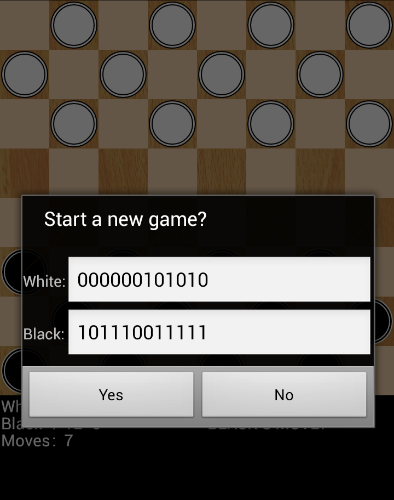
\includegraphics[width=\textwidth]{dialog}
\label{fig:dialogBoite}
\caption{Boîte de dialogue}
\end{subfigure}~
\begin{subfigure}{.4\textwidth}
\centering
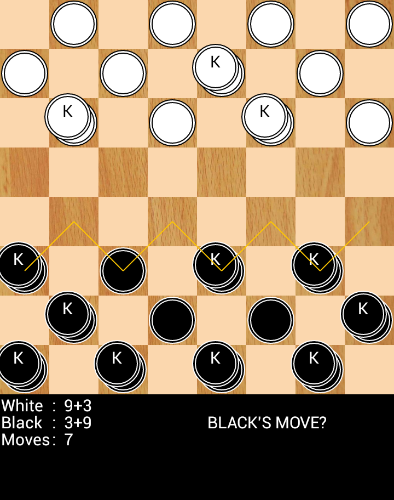
\includegraphics[width=\textwidth]{dialog2}
\label{fig:dialogPlacement}
\caption{Initialisation du plateau}
\end{subfigure}
\label{fig:dialog}
\caption{Placement des pions}
\end{figure}

Pour ce faire, l'idée était de faire un vrai projet Android pour pouvoir créer et tester facilement une boîte de dialogue, puis d'exporter le projet en \mytexttt{.apk}, décompiler cet \mytexttt{.apk}, récupérer le code de la boîte de dialogue dans le fichier \mytexttt{.smali} correspondant, et le mettre à la place du code de la vraie boîte de dialogue du jeu.

Nous avons donc fait un projet Android contenant les classes \mytexttt{b} (listing \ref{lstPlacementB}) et \mytexttt{a} (listing \ref{lstPlacementA}), ainsi qu'une classe \mytexttt{MainActivity} présente uniquement pour pouvoir lancer l'application et tester la boîte de dialogue. La classe \mytexttt{b} correspond à la classe \mytexttt{CheckersView} qui est la vue du jeu, et la classe \mytexttt{a} correspond à la classe \mytexttt{CheckersController} qui est le contrôleur. \`{A} noter que certaines lignes de la classe \mytexttt{b} ont été retirées (comme l'affectation du layout pour les éléments de la boîte de dialogue ou le constructeur) afin de la simplifier.\\

On peut remarquer plusieurs choses. Tout d'abord, nous avons gardé les noms des packages, classes, variables ainsi que les signatures des fonctions tels qu'ils apparaissent dans les fichiers \mytexttt{.smali} du jeu pour pouvoir injecter notre code sans trop de problèmes. Par contre, pour les fonctions et variables supplémentaires qui ne sont utilisées que par notre code, nous avons mis des vrais noms puisque ça ne pose pas de problème.

Ensuite, la méthode \mytexttt{a} de la classe \mytexttt{b} ne fait que retourner \mytexttt{false}. Cette méthode est uniquement présente pour pouvoir compiler le code puisque l'on doit y faire appelle quand l'utilisateur confirme la nouvelle partie. Quant à la méthode \mytexttt{a} de la classe \mytexttt{a} qui doit initialiser le plateau, elle ne contient que le code à compiler et à injecter dans la méthode originale.\\

Pour entrer plus en détail dans le code, et plus précisément la classe \texttt{b}, on a les quatres variables \mytexttt{newGame(White|Black)(Pieces|Kings)Placement} (ligne 9) qui contiennent les positions des pions normaux et des dames pour les deux joueurs. On peut voir que, par défaut, la variable \mytexttt{newGameWhitePiecesPlacement} contient un entier avec les douzes premiers bits à `1', et que la variable \mytexttt{newGameBlackKingsPlacement} contient un entier avec les douzes derniers bits `1'.

Le jeu utilise des entiers pour représenter le plateau. Les douzes premiers bits correspondent aux trois premières rangées, les douzes derniers aux trois dernières, le premier bit est la case tout en haut à gauche, et le dernier est la case tout en bas à droite. C'est pour ça que l'on fait des opérations étranges (ligne 50 et lignes 64 à 69) sur la saisie de l'utilisateur.

Pour ce qui est de la classe \texttt{a}, on assigne simplement les valeurs de nos variables aux vraies positions des pions avant l'initialisation du plateau (lignes 14 à 17).\\

Une fois notre \texttt{.apk} généré et le code de notre application Android décompilé, on peut très simplement injecter notre code dans les \texttt{.smali} du jeu.\\

\begin{lstlisting}[caption=b.java (CheckersView.java), label=lstPlacementB]
package com.xxogli.xadroid.checkers;

// CheckersView
public class b extends View {

	private Context a;
	private a p;		// CheckersController
	
	public int newGameWhitePiecesPlacement = 4095;
	public int newGameWhiteKingsPlacement = 0;
	public int newGameBlackPiecesPlacement = 0;
	public int newGameBlackKingsPlacement = -1048576;

	private TextView textView(String s) {
		TextView tv = new TextView(a);
		tv.setText(s);
		return tv;
	}
	
	private EditText editText(String s) {
		EditText et = new EditText(a);
		et.setText(s);
		return et;
	}
	
	private TableRow tableRow(String s, EditText et) {
		TableRow tr = new TableRow(a);
		tr.addView(textView(s));
		tr.addView(et);
		return tr;
	}
	
	private TableLayout tableLayout(TableRow ...rows) {
		TableLayout tl = new TableLayout(a);
		for(TableRow tr : rows) {
			tl.addView(tr);
		}
		return tl;
	}
	
	private LinearLayout linearLayout(View ...views) {
		LinearLayout ll = new LinearLayout(a);
		for(View v : views) {
			ll.addView(v);
		}
		return ll;
	}

	private int value(EditText et) {
		return Integer.parseInt(new StringBuilder(et.getText().toString()).reverse().toString(), 2);
	}
	
	// newGameDialog
	public void f() {
		AlertDialog.Builder b = new AlertDialog.Builder(a);
		final EditText et1 = editText("000000000000");
		final EditText et2 = editText("000000000000");
		b.setView(tableLayout(
			tableRow("White:", et1), tableRow("Black:", et2)
		)).setMessage("Start a new game?")
		.setCancelable(false)
		.setPositiveButton("Yes", new OnClickListener() {
			public void onClick(DialogInterface dialog, int which) {
				int i = value(et1);
				newGameWhitePiecesPlacement = ~i & 0xFFF;
				newGameWhiteKingsPlacement = i & 0xFFF;
				i = value(et2) << 20;
				newGameBlackPiecesPlacement = ~i & 0xFFF00000;
				newGameBlackKingsPlacement = i & 0xFFF00000;
				a(false, -1, 0, 0, 0);
				postInvalidate();
			}
		})
		.setNegativeButton("No", new OnClickListener() {
			public void onClick(DialogInterface dialog, int which) {
			}
		}).show();
	}
	
	// gameStatus
	private final boolean a(boolean b, int m, int v, int d, int n) {
		return false;
	}

}
\end{lstlisting}

\begin{lstlisting}[caption=a.java (CheckersController.java), label=lstPlacementA]
package com.xxogli.xadroid.checkers;

// CheckersController
public class a {

	private b j;		// CheckersView
	private int d;	// lastWhitePiecesPlacement
	private int e;	// lastWhiteKingsPlacement
	private int f;	// lastBlackPiecesPlacement
	private int g;	// lastBlackKingsPlacement

	// initPlateau
	public final void a() {
		this.d = j.newGameWhitePiecesPlacement;
		this.e = j.newGameWhiteKingsPlacement;
		this.f = j.newGameBlackPiecesPlacement;
		this.g = j.newGameBlackKingsPlacement;
	}

}
\end{lstlisting}